\chapter{Algebra di Boole}
\label{cha:AlgebradiBoole}
\minitoc
\mtcskip                                % put some skip here
\minilof                                % a minilof
\mtcskip                                % put some skip here
\minilot
\FloatBarrier
\section{Variabili e funzioni booleane}
\label{sec:VariabiliBooleane}
Una variabile booleana\index{Variabile!booleana} è una variabile che può assumere solo due valori, che possono essere indicati o  con\nobs$0$\nobs e\nobs$1$ o con $basso$\nobs e\nobs$alto$, con $vero$\nobs o \nobs$falso$. Nella realtà, a questi valori sono  associati valori arbitrari es: $+5\si{\volt}$ $-5\si{\volt}$, $+12\si{\volt}$ $-12\si{\volt}$. 

 Un sistema si trova in un determinato stato a seconda del valore che assumono le variabili booleane associate.   Vi sono due variabili  particolari la variabile\nobs$0$ che assume solo il valore\nobs$0$ e la variabile \nobs$1$ che assume solo il valore\nobs$1$. 

Una funzione (operazione) booleana\index{Funzione!booleana} è una relazione  che ha in ingresso delle variabili indipendenti e in uscita una variabile dipendente.

A ogni sistema è associata una tabella detta tavola di verità\index{Tavola di verità}. Una tavola di verità rappresenta in forma tabellare, in base agli stati del sistema in entrata, lo stato del sistema in uscita. Si può facilmente provare %, utilizzando la tavola~\vref{tab:statisistema},  
che la tabella\vref{tab:totfunzzionilogiche} rappresenta tutte le funzioni logiche con due valori in entrata.

Due funzioni logiche sono equivalenti\index{Funzione!booleana!equivalente} se hanno la stessa tavola di verità. Esempio di questo sono la tabella\nobs\vref{tab:tabVeritaEOR} e la tabella\nobs\vref{tab:tabVeritaEOR2} che sono fra di loro equivalenti. 

Un metodo grafico per rappresentare una funzione logica  è il circuito che si ottiene combinando i simboli  elencati nella tabella\nobs\vref{tab:Portelogichetavver}. Un esempio di ciò sono  i due circuiti\nobs\vref{Tab:circuito2e3} che rappresentano entrambi la funzione $XOR$\index{Funzione!booleana!XOR}  ottenuta come combinazione di $AND$\index{Funzione!booleana!AND} e $OR$\index{Funzione!booleana!OR}

Principio di dualità: Se una funzione logica è vera, allora è vera la funzione che si ottiene scambiando $AND$ con  $OR$ e  $0$ con $1$ e viceversa.

\begin{table} %[H]
	%\centering
	\begin{tabular}{cccccccccccccccccc}
	\toprule
	A & B & $0$ & NOR & $\overline{A}$ &  &  & $\overline{B}$ & XOR & NAND & AND & XNOR &  & B & A &  & OR & $1$ \\ 
	\midrule
	1 & 1 & 0 & 0 & 0 & 0 & 0 & 0 & 0 & 0 & 1 & 1 & 1 & 1 & 1 & 1 & 1 & 1 \\ 
	1 & 0 & 0 & 0 & 0 & 0 & 1 & 1 & 1 & 1 & 0 & 0 & 0 & 0 & 1 & 1 & 1 & 1 \\ 
	0 & 1 & 0 & 0 & 1 & 1 & 0 & 0 & 1 & 1 & 0 & 0 & 1 & 1 & 0 & 0 & 1 & 1 \\ 
	0 & 0 & 0 & 1 & 1 & 0 & 0 & 1 & 0 & 1 & 0 & 1 & 1 & 0 & 0 & 1 & 0 & 1 \\ 
	\bottomrule
	\end{tabular}
	\caption{Funzioni logiche}
	\label{tab:totfunzzionilogiche}
\end{table}
\subsection{Esempi}
\label{sec:Esempiofunzlog}
Definire, utilizzando le funzioni logiche:

$tavolo=(legno,ferro,3gambe,4gambe,piano)$,

$auto=(3 porte,5 porte,ruote,motore)$, 

$penna=(sfera,stilografica,rossa,nera,verde,cancellabile,indelebile)$

Una cassaforte ha quattro lucchetti, x, y, v, w, che devono essere tutti aperti affinché la
cassaforte si apra.  Tre persone A, B, C,  hanno le  chiavi. A possiede le chiavi v e y; 
B ha le chiavi v e x e C tiene w e y. Le variabili A, B, C sono uguali a uno se la persona corrispondente è presente, altrimenti sono uguali a zero. Costruire la tavola
della verità della funzione $Y=f(A,B,C)$. La funzione  vale uno se e solo se la cassaforte può essere  aperta,
 esprimere f in forma algebrica. Per risolvere almeno la prima parte dell'esercizio costruiamo una tabella  che leghi le chiavi alle tre persone.
\begin{table}
	    \centering
		\begin{tabular}{c|cccc}
			& \textbf{x} & \textbf{y} &\textbf{v}& \textbf{w}\\
			\toprule 
			\textbf{A} &  & \textbullet &\textbullet & \\ 
			\textbf{B} & \textbullet &  & \textbullet& \\ 
			\textbf{C} &  & \textbullet & & \textbullet\\ 
			\bottomrule
		\end{tabular}
	\caption[]{Persone e chiavi}
	\label{tab:personeechiavi}
\end{table} 
Quindi: il sistema (la cassaforte aperta o chiusa), dipende da tre variabili $A$, $B$ e $C$ che assumono solo due valori $1$ se la chiave è presente o $0$ altrimenti. In uscita $Y$ può assumere due valori $1$ se la cassaforte è aperta o $0$ nell'altro caso. 

La tabella~\vref{tab:personeechiavi} permette di costruire la tavola di verità\nobs\vref{tab:tavolaveritacasaforte} della funzione. La tabella, dipendendo da tre variabili in ingresso, ha otto stati. Iniziamo a costruire la tavola di verità del sistema. Nella prima riga abbiamo che $A=0$, $B=0$ e $C=0$, poiché nessuna chiave è presente, la cassaforte rimane chiusa quindi $Y=0$. Nella seconda riga abbiamo che $A=0$, $B=0$ e $C=1$,  due chiavi sono presenti ma \nobs\vref{tab:personeechiavi} ci dice che queste non bastano e la cassaforte è chiusa e quindi $Y=0$. Il discorso è analogo  per le righe rimanenti. Nella riga quattro abbiamo che $A=0$, $B=1$ e $C=1$  sono presenti quattro chiavi e la cassaforte viene aperta per cui $Y=1$.  Stesso discorso la riga otto e anche in questo caso $Y=1$.
\begin{table}
		\centering
\begin{tabular}{c|c|c|c|c}
	& \textbf{A} & \textbf{B} & \textbf{C} & \textbf{Y} \\
	\toprule 
	1& 0 & 0 & 0 & 0 \\ 
	2& 0 & 0 & 1 &  0\\ 
	3& 0 & 1 & 0 &  0\\ 
	4& 0 & 1 & 1 &  1\\ 
	5& 1 & 0 & 0 &  0\\ 
	6& 1 & 0 & 1 &  0\\ 
	7& 1 & 1 & 0 &  0\\ 
	8& 1 & 1 & 1 &  1\\ 
	\bottomrule
\end{tabular} 
	\caption{Tavola di verità}
	\label{tab:tavolaveritacasaforte}
\end{table}
\section{Tavole di verità}
\label{sec:TavoleDiVeritA}
\begin{figure} %[H]
\centering
	\pagestyle{empty}
	% Set the overall layout of the tree
\tikzstyle{level 1}=[level distance=3.5cm, sibling distance=3.5cm]
\tikzstyle{level 2}=[level distance=3.5cm, sibling distance=2cm]
\tikzstyle{level 3}=[level distance=3cm, sibling distance=0.8cm] 
% Define styles for bags and leafs
%\tikzstyle{bag} = [text width=4em, text centered]
\tikzstyle{bag} =[shape=circle,draw,
text centered]
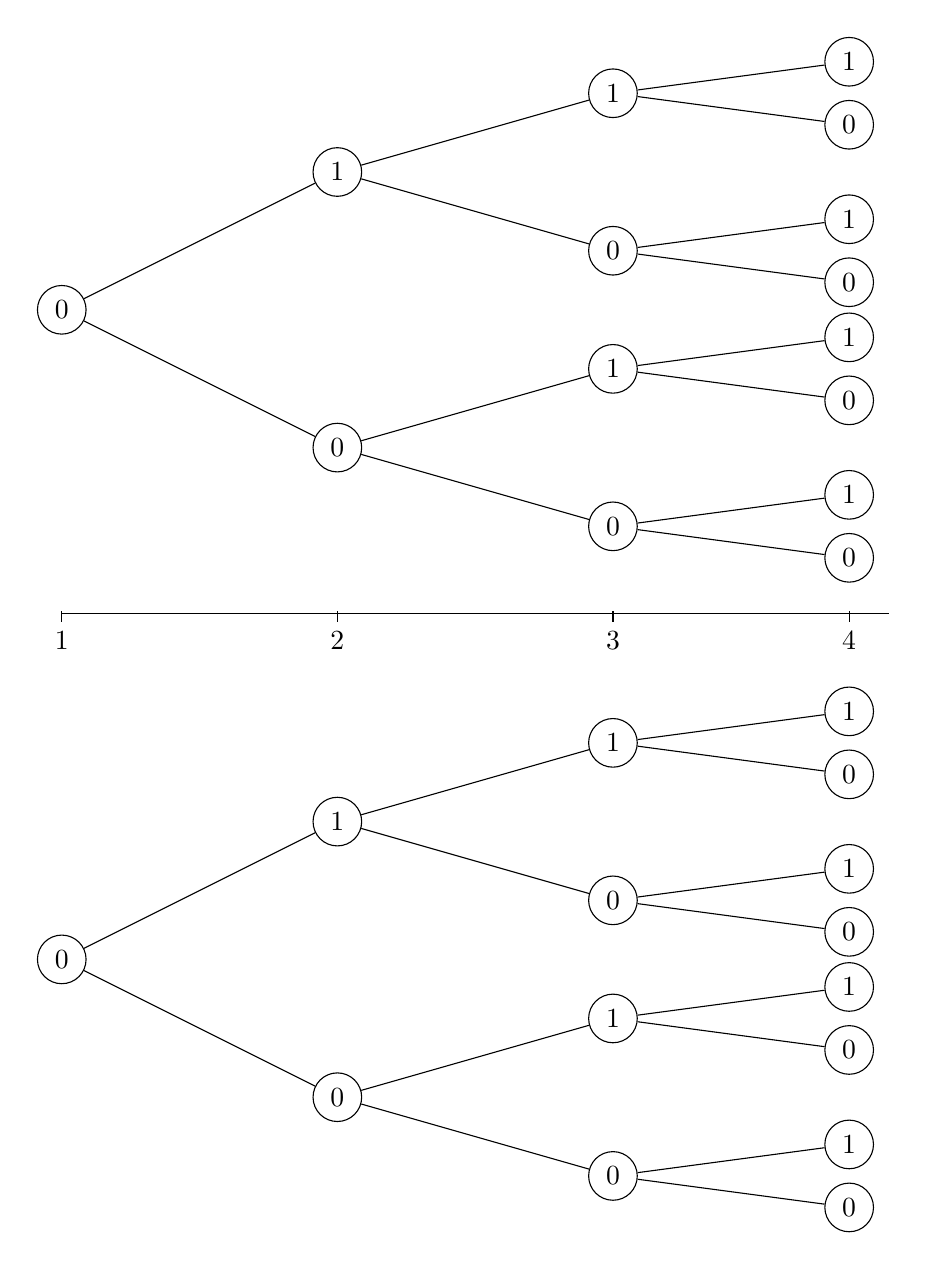
\begin{tikzpicture}[grow=right, sloped]
\matrix [row sep=1em] 
{
	\node[bag] {0}
	child{   
		node[bag] {0}
		child{
			node[bag] {0}
			child{
				node[bag]{0}
			}
			child{
				node[bag]{1}
			}
		}
		child {
			node[bag] {1}
			child{
				node[bag]{0}
			}
			child{
				node[bag]{1}
			}		
		}
	}
	child{
		node[bag]{1}
		child{
			node[bag] {0}
			child{
				node[bag]{0}
			}
			child{
				node[bag]{1}
			}
		}
		child {
			node[bag] {1}
			child{
				node[bag]{0}
			}
			child{
				node[bag]{1}
			}
		}   
	};
	&\\
	\draw (0,0) --  (10.5,0);
	\draw (0.0,1pt) -- (0.0,-3pt)
	node[anchor=north] {1};
	\draw (3.5,1pt) -- (3.5,-3pt)
	node[anchor=north] {2};
	\draw (7,1pt) -- (7,-3pt)
	node[anchor=north] {3};
	\draw (10,1pt) -- (10,-3pt)
	node[anchor=north] {4};\\
	\node[bag] {0}
	child{   
		node[bag] {0}
		child{
			node[bag] {0}
			child{
				node[bag]{0}
			}
			child{
				node[bag]{1}
			}
		}
		child {
			node[bag] {1}
			child{
				node[bag]{0}
			}
			child{
				node[bag]{1}
			}		
		}
	}
	child{
		node[bag]{1}
		child{
			node[bag] {0}
			child{
				node[bag]{0}
			}
			child{
				node[bag]{1}
			}
		}
		child {
			node[bag] {1}
			child{
				node[bag]{0}
			}
			child{
				node[bag]{1}
			}
		}   
	};\\
};
\end{tikzpicture}
	\caption{Stati del sistema}
	\label{tab:statisistema}
\end{figure}

Le funzioni logiche sono divise in gruppi. Il primo è formato dalle funzioni AND\index{Funzione!booleana!AND}, OR\index{Funzione!booleana!OR} e NOT\index{Funzione!booleana!NOT}. Segue il gruppo formato solo da NAND\index{Funzione!booleana!NAND}. Infine quello composto solo  da NOR\index{Funzione!booleana!NOR}. Ogni gruppo è tale perché in grado di generare le rimanenti funzioni. La figura~\vref{tab:Portelogichetavver} riporta le tavole di verità di queste funzioni. 

Combinando fra di loro le funzioni  otteniamo altre funzioni come viene per esempio, nella tabella~\vref{tab:ComposizionePorte}. 

La tabella~\vref{tab:statisistema} da in verticale di quante righe deve avere una tavola di verità.  Con una variabile due righe,  due variabili  otteniamo quattro righe etc. Mentre in orizzontale,in base al numero delle variabili, percorrendo i grafi da sinistra verso destra, avremo tutti i possibili stati di un sistema.
\subsection{Funzione AND}
\label{sub:funzioneAND}
La funzione AND\index{Funzione!booleana!AND} ha due valori in entrata ed  un valore in uscita che è vero solo quando sono veri entrambi i valori in entrata. Il simbolo che la rappresenta l'operazione è il prodotto.

Nella realtà casi in cui si usano funzioni AND sono molteplici. In genere si usa una funzione AND\index{Funzione!booleana!AND} quando  si eseguono due azioni in contemporaneamente come per esempio nel dispositivi di azionamento di una pressa in cui si premono contemporaneamente due pulsanti in modo da impegnare entrambe le mani, evitando così incidenti. 

Un esempio della funzione AND\index{Funzione!booleana!AND} è il seguente circuito\nobs\vref{tab:elettricoAND}. Abbiamo un circuito con due pulsanti in serie.  La lampada si accende solo premendo solo contemporaneamente i due interruttori.
\begin{table}[H]
	\centering
	\begin{circuitikz} \draw
		(0,0)--(0,2)
		(5,0)--(5,2)
		(0,0) to[lamp] (2,0)
		(2,0) to[battery] (5,0)
		(0,2) to[opening switch] (3,2)
		(3,2) to[opening switch] (5,2);
	\end{circuitikz}
	\caption{Circuito AND}
	\label{tab:elettricoAND}
\end{table}
	
La tabella\nobs\ref{tab:Portelogichetavver} mostra la tavola di verità\index{Tavola di verità!AND} della $AND$\index{Funzione!booleana!AND} e il simbolo grafico associato.
\subsection{Funzione OR}
\label{sub:funzioneOR}
La funzione OR\index{Funzione!booleana!OR} ha due valori in entrata e un valore in uscita. Questo valore è vero quando almeno uno dei valori in ingresso è vero. Il simbolo che la rappresenta è la somma. 

Un esempio dell'uso della funzione OR\index{Funzione!booleana!OR} è l'impianto di illuminazione di una stanza in cui due interruttori distinti permettono di accendere una lampadina.

Un circuito in parallelo, come il circuito\nobs\vref{tab:ZunzioneOR}, rappresenta la funzione OR\index{Funzione!booleana!OR}. Per accendere la lampadina basta premere almeno un interruttore.
\begin{table}
	\centering
	\begin{circuitikz} \draw
		(0,0)--(0,2)
		(5,0)--(5,2)
		(0,0) to[lamp] (2,0)
		(2,0) to[battery] (5,0)
		(0,2)--(1,2)
		(1,1)--(1,3)
		(4,1)--(4,3)
		(4,2)--(5,2)
		(1,3) to[opening switch] (4,3)
		(1,1) to[opening switch] (4,1);
	\end{circuitikz}
	\caption{Circuito OR}
	\label{tab:ZunzioneOR}
\end{table}
La tabella\nobs\ref{tab:Portelogichetavver} mostra la tavola di verità\index{Tavola di verità!OR} della OR\index{Funzione!booleana!OR} e il simbolo grafico associato.
\subsection{Funzione NOT}
\label{sub:funzionenot}
La funzione NOT ha un solo valore in entrata e un solo valore in uscita. Il valore in uscita è l'opposto a quello in ingresso. Il simbolo che rappresenta l'operazione è un trattino che si pone sopra la variabile.

Un esempio dell'uso della funzione NOT\index{Funzione!booleana!NOT} è per esempio l'interruttore della luce di cortesia di un'auto che si accende aprendo la portiera.

Un circuito come il circuito\nobs\vref{tab:CircuitoNOT} rappresenta la funzione NOT. La tabella\nobs\ref{tab:Portelogichetavver} mostra la tavola di verità\index{Tavola di verità!NOT} della NOT e il simbolo grafico associato.
\begin{table}
	\centering
	 \begin{circuitikz} \draw
		(0,0)--(0,2)
		(6,0)--(6,2)
		(0,1) to[lamp] (6,1)
		(0,2)--(3,2)
		(3,2) to[battery,v_<=$+-$] (6,2)
		(0,0) to[opening switch] (3,0)
		(3,0) to[battery,v_<=$+-$] (6,0);
	\end{circuitikz}
	\caption{Circuito NOT}
	\label{tab:CircuitoNOT}
\end{table}
	
\subsection{Funzione XOR}
\label{sub:funzioneXOR}
La funzione XOR\index{Funzione!booleana!XOR} ha due valori in entrata ed un valore in uscita che è vero quando solo uno dei valori in ingresso è vero.

Il circuito\nobs\vref{tab:circuitoXOR} rappresenta un OR esclusivo. Sono due gruppi di pulsanti in parallelo messe in serie. La seconda serie di pulsanti sono i negati dei precedenti. Quando vien premuto il primo pulsante $A$ il pulsante $\overline{A}$ del secondo circuito viene aperto e viceversa, analogamente per il pulsante $B$. In questo circuito la corrente passa e  lampadina si accende, solo se è premuto un solo pulsante ma non entrambi.

La tabella\nobs\ref{tab:Portelogichetavver} mostra la tavola di verità della XOR\index{Tavola di verità!XOR} e il simbolo grafico associato.
\begin{table} %[H]
		\centering
		\begin{circuitikz} \draw
			(0,0)--(0,2)
			(7,0)--(7,2)
			(0,0) to[lamp] (3,0)
			(3,0) to[battery] (7,0)
			(0,2)--(1,2)
			(1,1)--(1,3)
			(3,1)--(3,3)
			(3,2)--(4,2)
			(4,1)--(4,3)
			(6,1)--(6,3)
			(6,2)--(7,2)
			(1,3) to[opening switch=$A$] (3,3)
			(1,1) to[opening switch=$B$] (3,1)
			(4,1) to[closing switch=$\overline{B}$] (6,1)
			(4,3) to[closing switch=$\overline{A}$] (6,3);
		\end{circuitikz}
	\caption{Circuito XOR}
	\label{tab:circuitoXOR}
	\end{table}
\subsection{Funzione NAND}
\label{sub:funzioneNAND}
La funzione NAND\index{Funzione!booleana!NAND} ha due valori in entrata ed ha un valore in uscita che è falso solo quando sono veri entrambi i valori in entrata.

La tabella\nobs\ref{tab:Portelogichetavver} mostra la tavola di verità\index{Tavola di verità!NAND} della $NAND$\index{Funzione!booleana!NAND} e il simbolo grafico associato. La $NAND$ è la negazione di $AND$\index{Funzione!booleana!AND}.

\subsection{Funzione NOR}
\label{sub:funzioneNOR}
La funzione NOR\index{Funzione!booleana!NOR} ha due valori in entrata ed ha un valore in uscita che è vero solo quando sono falsi entrambi i valori in entrata.

La tabella\nobs\ref{tab:Portelogichetavver} mostra la tavola di verità\index{Tavola di verità!NOR} della NOR\index{Funzione!booleana!NOR} e il simbolo grafico associato. La NOR è la negazione di OR 
\subsection{Funzione XNOR}
\label{sub:funzioneXNOR}
La funzione XNOR\index{Funzione!booleana!XNOR} ha due valori in entrata ed ha un valore in uscita che è vero solo quando sono falsi entrambi i valori in entrata o quando sono entrambi veri. 

La tabella\nobs\ref{tab:Portelogichetavver} mostra la tavola di verità\index{Tavola di verità!XNOR} della XNOR e il simbolo grafico associato. La XNOR è la negazione di XOR 

Il circuito\nobs\vref{tab:circuitoXNOR} è formato da due blocchi di pulsanti in serie messi in parallelo. Quando vien premuto il primo pulsante $A$ il pulsante $\overline{A}$ del secondo circuito viene aperto e viceversa, analogamente per il pulsante $B$. La lampadina si accende o quando entrambi i pulsanti $A$ e $B$ sono premuti o entrambi i  pulsanti $A$ e $B$ sono tenuti alzati.
\begin{table}[H]
	\centering
	\begin{circuitikz} \draw
		(0,0)--(0,2)
		(7,0)--(7,2)
		(0,0) to[lamp] (3,0)
		(3,0) to[battery] (7,0)
		(0,2)--(1,2)
		(1,1)--(1,3)
		(6,1)--(6,3)
		(6,2)--(7,2)
		(1,3) to[opening switch=$A$] (4,3)
		(4,3) to[opening switch=$B$] (6,3)
		(1,1) to[closing switch=$\overline{A}$] (4,1)
		(4,1) to[closing switch=$\overline{B}$] (6,1);
	\end{circuitikz}
	\caption{Circuito XNOR}
	\label{tab:circuitoXNOR}
\end{table}
Come si è detto a una funzione logica è possibile associare una tavola di verità\index{Tavola di verità!Costruire}. Un esempio di costruzione  è la tabella~\vref{tab:tabVeritaEOR}. Il metodo usato è molto semplice,  prevede di suddividere la funzione nelle sue componenti e risolverle partendo da sinistra verso destra. Questo deve essere fatto rispettando le convenzioni di precedenza, cioè le negazioni (funzione NOT), poi i prodotti (Funzione AND\index{Funzione!booleana!AND}), e infine le somme (Funzione OR\index{Funzione!booleana!OR}).Possiamo cambiare le  precedenze mettendo fra  delle parentesi le operazioni che devono essere eseguite prima.
In conclusione, abbiamo parlato di tavola di verità\index{Tavola di verità}, circuito, funzione logica, che sono concetti fra loro equivalenti\vref{tab:FunzioneTavolaCircuito} e fra loro connessi.
\begin{table} 
	\centering
	\begin{tikzpicture}[very thick,node distance=5cm,text centered,minimum size=3cm]
		\node [circle, draw] (a) {Funzione logica};
		\node [circle, draw] (b) [above right=of a] {Tavola di verità};
		\node [circle, draw] (c) [above left=of a]{Circuito};
		\draw [<->] (a) to (b);
		\draw [<->] (b) to (c);
		\draw [<->] (c) to (a);
	\end{tikzpicture}
	\caption{Funzione, Tavola e Circuito}
	\label{tab:FunzioneTavolaCircuito}
\end{table}
\begin{table}
	\centering
	\begin{tabular}{@{}cc@{\hspace{2cm}}cc@{}}
	\begin{truthtable}{AND}
	\toprule
	$A$&$B$&$AB$\\
	\midrule           
	0&0&0\\
	1&0&0\\
	0&1&0\\
	1&1&1\\
	\bottomrule
	\end{truthtable}
	& \cport{and} &
	\begin{truthtable}{NAND}
	\toprule
	$A$&$B$&$A\mathbin{\overline{\wedge}}B$\\
	\midrule
	0&0&1\\
	1&0&1\\
	0&1&1\\
	1&1&0\\
	\bottomrule
	\end{truthtable}
	& \cport{nand} \\
	\addlinespace[3ex]
	\begin{truthtable}{OR}
	\toprule
	$A$&$B$&$A+B$\\
	\midrule         
	0&0&0\\
	1&0&1\\
	0&1&1\\
	1&1&1\\
	\bottomrule
	\end{truthtable}
	& \cport{or} &
	\begin{truthtable}{NOR}
	\toprule
	$A$&$B$&$A\mathbin{\overline{\vee}}B$\\
	\midrule
	0&0&1\\
	1&0&0\\
	0&1&0\\
	1&1&0\\
	\bottomrule
	\end{truthtable}
	& \cport{nor} \\
	\addlinespace[3ex]
	\begin{truthtable}{XOR}
	\toprule
	$A$&$B$&$A\XOR B$\\
	\midrule         
	0&0&0\\
	1&0&1\\
	0&1&1\\
	1&1&0\\
	\bottomrule
	\end{truthtable}
	& \cport{xor} &
	\begin{truthtable}{XNOR}
	\toprule
	$A$&$B$&$A\mathbin{\overline{\XOR}}B$\\
	\midrule
	0&0&1\\
	1&0&0\\
	0&1&0\\
	1&1&1\\
	\bottomrule
	\end{truthtable}
	& \cport{xnor} \\
	\addlinespace[3ex]
	\multicolumn{4}{c}{%
		\begin{tabular}{@{}cc@{}}
		\begin{truthtable}[2]{NOT}
		\toprule
		$A$&$\overline{A}$\\
		\midrule         
		0&1\\
		1&0\\
		\bottomrule
		\end{truthtable}
		& \cport{not}
		\end{tabular}}
	\end{tabular}
	\caption{Porte logiche}
	\label{tab:Portelogichetavver}
\end{table} 
\begin{table} %[H]
	\centering
	\begin{tabular}{ccc}
	\toprule
	\begin{circuitikz} \draw
	(0,0) node[and port] (myand) {}
	(1,0) node[not port] (mynot) {}
	(myand.out) -- (mynot.in)
	;\end{circuitikz}&&\begin{circuitikz} \draw
	(0,0) node[nor port]  {}
	;\end{circuitikz} \\
	AND +  NOT &=&NAND \\
	\midrule
	\begin{circuitikz} \draw
	(0,0) node[or port] (myor) {}
	(1,0) node[not port] (mynot) {}
	(myor.out) -- (mynot.in)
	;\end{circuitikz}&& \begin{circuitikz} \draw
	(0,0) node[nor port]  {}
	;\end{circuitikz} \\
	OR +  NOT &=&NOR  \\ 
	\midrule
	\begin{circuitikz} \draw
	(0,0) node[xor port] (myxor) {}
	(1,0) node[not port] (mynot) {}
	(myxor.out) -- (mynot.in)
	;\end{circuitikz}&& \begin{circuitikz} \draw
	(0,0) node[xnor port]  {}
	;\end{circuitikz} \\
	XOR +  NOT &=&XNOR  \\ 
	\bottomrule
	\end{tabular} 
	\caption{Composizione porte}%
	\label{tab:ComposizionePorte}%
\end{table}
\section{Proprietà dell'algebra algebra booleana}
\label{sec:Algebrabooleana}
La tabella\nobs\vref{Tab:AlgebrAbOOLEAN} elenca le principali proprietà delle funzioni AND\index{Funzione!booleana!AND} e OR\index{Funzione!booleana!OR} e mostra come le proprietà delle funzioni siano legate tramite il principio di dualità. Infatti, osservando la tabella si vede come le proprietà elencate a sinistra trovino il loro corrispondente duale a destra e viceversa. La tabella\nobs\vref{Tab:funzlogSemp} mostra come ottenere i risultati. Non vengono dimostrate tutte le relazioni inquarto le altre si ottengono per dualità.

%\altapriorita{Specificare meglio}
Una funzione logica non è unica ma può essere scritta in modi fra di loro equivalenti. La tabella\nobs\vref{Tab:funzlogSemp} mostra come con pochi passaggi si può passare da una funzione logica a una equivalente.
\begin{table}%[H]
\centering
\begin{tabular}{lcl}
\toprule
&PROPRIET\'A&\\
&$\overline{\overline{A}}=A$&\\
$A+0=A$&Elemento neutro&$A\cdot1=A$\\
$A+1=1$&Assorbimento&$A\cdot0=0$\\
$A+A=A$&Idempotenza&$A\cdot A=A$\\
$A+\overline{A}=1$&&$A\cdot\overline{A}=0$\\
$A+B=B+A$&Commutativa&$A\cdot B=B\cdot A$\\
$(A\cdot B)\cdot C=A\cdot(B\cdot C)=A\cdot B\cdot C$&Associativa&$(A+B)+C=A+(B+C)=A+B+C$\\
\midrule
&TEOREMI&\\
\midrule
$A+A\cdot B=A$&&$A\cdot(A+B)=A$\\
$A+\overline{A}\cdot B=A+B$&&$A\cdot (\overline{A}+B)=AB$\\
$(A+B)\cdot(A+C)=A+B\cdot C$&&$A\cdot B+A\cdot C=A\cdot(B+C)$\\
$(A+B)\cdot(\overline{A}+C)=\overline{A}\cdot B+A\cdot C$&&$A\cdot B+\overline{A}\cdot C=(\overline{A}+B)\cdot(A+B)$\\
\midrule
&TEOREMI DI DE MORGAN&\\
\midrule
$\overline{A+B}=\overline{A}\cdot\overline{B}$&&$\overline{A\cdot B}=\overline{A}+\overline{B}$\\
\bottomrule
\end{tabular}
\caption{Teoremi e proprietà algebra di Boole}%
\label{Tab:AlgebrAbOOLEAN}%
\end{table}
\begin{table}
\centering
\begin{tabular}{lcl}
\toprule
%\midrule
PROPRIET\'A&&DIMOSTRAZIONE\\
\midrule
$A+A\cdot B=A$&&$A+A\cdot B=$\\
&&$=A\cdot(1+B)=$\\
&&$=A\cdot1=A$\\ 
\midrule
$A+\overline{A}\cdot B=A+B$&&$A+A\cdot B+\overline{A}\cdot B=$\\
&&$=A+(A+\overline{A})\cdot B=$\\
&&$=A+1\cdot B=$\\
&&$=A+B$\\
\midrule
$(A+B)\cdot(A+C)=A+B\cdot C$&&$(A+B)\cdot(A+C)=$\\
&&$A\cdot A+A\cdot C+A\cdot B+B\cdot C=$\\
&&$=A+A\cdot C+A\cdot B+B\cdot C=$\\
&&$=A\cdot(1+C) +A\cdot B+B\cdot C=$\\
&&$=A\cdot 1 +A\cdot B+B\cdot C=$\\
&&$=A\cdot(1+B)+B\cdot C=$\\
&&$A+B\cdot C$\\
\midrule
$(A+B)\cdot(\overline{A}+C)=\overline{A}\cdot B+A\cdot C$&&$(A+B)\cdot(\overline{A}+C)$\\
&&$\overline{A}\cdot A+ A\cdot C +\overline{A}\cdot B+B\cdot A\cdot C$\\
&&$A\cdot B+\overline{A}\cdot B+B\cdot C$\\
&&$(A+B)\cdot C+\overline{A}\cdot B$\\
&&$(A+\overline{A}\cdot B)\cdot C+\overline{A}\cdot B$\\
&&$A\cdot C+\overline{A}\cdot B\cdot C+\overline{A}\cdot B$\\
&&$A\cdot C+\overline{A}\cdot B(C+1)$\\
&&$A\cdot C+\overline{A}\cdot B$\\
\bottomrule
\end{tabular}
\caption{Semplificazioni}
\label{Tab:funzlogSemp}
\end{table}
\section{Trovare la tavola di verità di una funzione}
\label{sec:Trovaretavolaveritàfunzione}
Per trovare data una funzione, la tavola di verità\index{Tavola di verità}, basta sostituire alle variabili booleane  i valori in ingresso e vedere cosa ha la funzione in uscita. 

Consideriamo la funzione $Y=A\cdot\overline{B}+\overline{A}\cdot B$  possiamo costruire la tabella\nobs\vref{tab:tabVeritaEOR} che fornisce tutti i calcoli necessari. Si procede sostituendo alle variabili tutti i valori possibili e ottenendo dopo i calcoli i risultati della colonna sette 

Analogo ragionamento è per $Y=(A+B)\cdot(\overline{A}+\overline{B})$ e ottenere la tabella\nobs\vref{tab:tabVeritaEOR2}.

Per $Y=\overline{A}\cdot\overline{B}\cdot C+\overline{A}\cdot B\cdot\overline{C}+\overline{A}\cdot B\cdot C+A\cdot B\cdot C$ otteniamo la tavola di verità\nobs\vref{Tab:esempio2bool}\index{Tavola di verità}

La tavola di verità per $Y=\overline{A}\cdot (A+B)+\overline{C}+B\cdot C$ e per $Y=B+\overline{C}$ è\nobs\vref{Tab:Tabveres1}
\begin{table}
	\centering
	\begin{tabular}{ccccccccccc}
		\toprule
		\multicolumn{10}{c}{$A\cdot\overline{B}+\overline{A}\cdot B$} \\ 
		&  &  & 1 & 3 & 2 & 7 & 4 & 6 & 5 \\ 
		A & B &  & $A$&$\cdot$  &$\overline{B}$&$+$& $\overline{A}$ &$\cdot$ &$B$  \\ 
		\cmidrule{1-2}\cmidrule{4-10}
		1 & 1 &  & 1 & 0 & 0 & 0 & 0 & 0 & 1 \\ 
		1 & 0 &  & 1 & 1 & 1 & 1 & 0 & 0 & 0 \\ 
		0 & 1 &  & 0 & 0 & 0 & 1 & 1 & 1 & 1 \\ 
		0 & 0 &  & 0 & 0 & 1 & 0 & 1 & 0 & 0 \\ 
		\bottomrule
	\end{tabular}
	\caption[]{Tavola di verità di $A\cdot\overline{B}+\overline{A}\cdot B$}
	\label{tab:tabVeritaEOR}
\end{table}
\begin{table}
	\centering
	\begin{tabular}{ccccccccccc}
		\toprule
		\multicolumn{10}{c}{$(A+B)\cdot(\overline{A}+\overline{B})$} \\ 
		&  &  & 1 & 3 & 2 & 7 & 4 & 6 & 5 \\ 
		A & B &  & $(A$&$+$  &$B)$ &$\cdot$ &$(\overline{A}$&$+$&$\overline{B})$  \\ 
		\cmidrule{1-2}\cmidrule{4-10}
		1 & 1 &  & 1 & 1 & 1 & 0 & 0 & 0 & 0 \\ 
		1 & 0 &  & 1 & 1 & 0 & 1 & 0 & 1 & 1 \\ 
		0 & 1 &  & 0 & 1 & 1 & 1 & 1 & 1 & 0 \\ 
		0 & 0 &  & 0 & 0 & 0 & 0 & 1 & 1 & 1 \\ 
		\bottomrule
	\end{tabular}
	\caption[]{Tavola di verità di $(A+B)\cdot(\overline{A}+\overline{B})$}
	\label{tab:tabVeritaEOR2}
\end{table}
\section{Trovare la funzione data la tavola di verità}
\label{sec:Trovarefunzionedatatavolaverità}
Per trovare la funzione, nota la tavola di verità\index{Tavola di verità!trovare!funzione}, possiamo utilizzare due metodi\footnote{I due metodi sono duali come si nota leggendo di seguito} 
\subsection{Somma di prodotti canonici} 
Per trovare data la tavola di verità la funzione si usa il metodo della somma di prodotti canonici\index{Somma prodotti canonici!\see{Mintermini}}. Ogni funzione logica si può scrivere come somma di prodotti detti mintermini\index{Mintermini}. Questi prodotti sono costituiti da prodotti di tutte le variabili in forma diretta o negata. Ogni mintermine assume il valore logico 1.

Nell'esempio uno si inizia dalla tavola\nobs\vref{Tab:esempio2bool},  si individuano le righe che hanno come risultato uno e si costruisce la somma dei mintermini. Nella riga due della tavola di verità si ha come risultato uno. Dato che le variabili $A$ $B$ assumono valore zero nel prodotto si inserisce il loro complemento e otteniamo $\overline{A}\cdot \overline{B}\cdot C$.

Si continua con lo stesso criterio ed otteniamo\[Y=2+3+4+8=\overline{A}\cdot\overline{B}\cdot C+\overline{A}\cdot B\cdot\overline{C}+\overline{A}\cdot B\cdot C+A\cdot B\cdot C\] cioè la funzione associata.
\begin{table}
	\centering
	\begin{tabular}{lccc|c}
		&A&B&C&Y\\
		\toprule
		1&0&0&0&0\\
		2&0&0&1&\textbf{1}\\
		3&0&1&0&\textbf{1}\\
		4&0&1&1&\textbf{1}\\
		5&1&0&0&0\\
		6&1&0&1&0\\
		7&1&1&0&0\\
		8&1&1&1&\textbf{1}\\
	\end{tabular}
	\caption[]{Tabella verità di $Y=\overline{A}\cdot\overline{B}\cdot C+\overline{A}\cdot B\cdot\overline{C}+\overline{A}\cdot B\cdot C+A\cdot B\cdot C$}
	\label{Tab:esempio2bool}
\end{table}
%\begin{table}
%	\begin{equation}
%	Y=2+3+4+8=\overline{A}\overline{B}C+\overline{A}B\overline{C}+\overline{A}BC+ABC
%	\end{equation}
%	\caption[]{Funzione booleana esempio 1}
%	\label{tab:esempio2funbool}
%\end{table}
\subsection{Prodotto di somme canoniche}
Per trovare, data la tavola di verità\index{Tavola di verità!trovare!funzione}, la funzione si usa il metodo della prodotti di somme  canoniche\index{Prodotti somme canoniche|see{Maxtermini} }. Ogni funzione logica si può scrivere come prodotto di somme detti maxtermini\index{Maxtermini}. Questi prodotti sono costituiti da somme di tutte le variabili in forma diretta o negata. Ogni maxtermine assume il valore logico 0.
Nell'esempio 1 si inizia dalla tavola\nobs\vref{Tab:esempio2bool}  si individuano le righe che hanno come risultato zero e si costruisce il prodotto dei maxtermini. Nella riga uno della tavola di verità si ha come risultato zero. Dato che le variabili $A$ $B$ $C$ assumono valore zero il max termine sarà $(A+B+C)$ 

Si continua con lo stesso criterio ed otteniamo\[Y=1+5+6+7=(A+B+C)(\overline{A}+B+C)(\overline{A}+B+ \overline{C})(\overline{A}+\overline{B}+C) \]
\section{Trovare il circuito corrispondente}
\label{Trovarecircuito}
\'E relativamente facile disegnare uno schema grafico che rappresenti un circuito. Partendo da \[Y=\overline{A}\cdot\overline{B}\cdot C+\overline{A}\cdot B\cdot\overline{C}+\overline{A}\cdot B\cdot C+A\cdot B\cdot C\] otteniamo\nobs\vref{tab:circuito1}. Il disegno è ottenuto ricordando le precedenza nelle operazioni per cui prima la negazione poi il prodotto e infine la somma.

I circuiti corrispondenti a \[(A+B)\cdot(\overline{A}+\overline{B})=A\cdot\overline{B}+\overline{A}\cdot B\] sono\nobs\vref{Tab:circuito2e3}
 In questo caso gli OR\index{Funzione!booleana!OR} hanno la precedenza perché contenuti in parentesi.
	
I circuiti corrispondenti a \[A\cdot B+\overline{A}\cdot\overline{B}=(\overline{A}+ B)\cdot(A+\overline{B})\] sono i circuiti disegnati in\nobs\vref{tab:circuito4e5}

Il circuito corrispondente a \[Y=\overline{A}\cdot (A+B)+\overline{C}+B\cdot C\] è il circuito disegnato in\nobs\vref{tab:circuito6}

Il circuito corrispondente a \[Y=\overline{A}\cdot C+\overline{A}\cdot B+B\cdot C\] è il circuito disegnato in\nobs\vref{tab:circuito7}
\begin{table}
\tikzstyle{branch}=[fill,shape=circle,minimum size=3pt,inner sep=0pt]
\centering
\begin{tikzpicture}
\node (A) at (0,0) {A};
\node (B) at (1,0) {B};
\node (C) at (2,0) {C};
\node[not gate US, draw] at ($(A)+(3,-2)$) (Not1) {};
\node[not gate US, draw] at ($(B)+(2,-1)$) (Not2) {};
\node[not gate US, draw] at ($(B)+(2,-2.5)$) (Not3) {};
\node[not gate US, draw] at ($(B)+(2,-3.4)$) (Not4) {};
\node[not gate US, draw] at ($(B)+(2,-3.9)$) (Not5) {};
\node[and gate US, draw, logic gate inputs=nnn, anchor=input 2] at ($(Not1.output-|Not2.output)+(1,.5)$) (and1){}; 
\node[and gate US, draw, logic gate inputs=nnn, anchor=input 3] at ($(Not3.output-|Not4.output)+(1,-.65)$) (and2){}; 
\node[and gate US, draw, logic gate inputs=nnn, anchor=input 3] at ($(Not5.output)+(1,-.4)$) (and3){}; 
\node[and gate US, draw, logic gate inputs=nnn, anchor=input 3] at ($(and3)+(-.4,-1.1)$) (and4){}; 
\node[or gate US, draw, logic gate inputs=nnnn, anchor=input 2] at ($(and2)+(3,-.5)$) (or1){};  
\draw (B)|-node[branch] {}(Not1.input);
\draw (A)|-node[branch] {}(Not2.input);
\draw(C)|-node[branch] {}(and1);
\draw(Not1.output)--([xshift=0.3cm]Not1.output) |-(and1.input 3);
\draw(Not2.output)--([xshift=0.3cm]Not2.output) |-(and1.input 1);
\draw (C)|-node[branch] {}(Not3.input);
\draw (A)|-node[branch] {}(Not4.input);
\draw(Not3.output)--([xshift=0.3cm]Not3.output) |-(and2.input 1);
\draw(Not4.output)--([xshift=0.3cm]Not4.output) |-(and2.input 3);
\draw(B)|-node[branch] {}(and2);
%
\draw(A)|-node[branch] {}(Not5.input);
\draw(Not5.output)--([xshift=0.3cm]Not5.output) |-(and3.input 1);
\draw(B)|-node[branch] {} (and3.input 2);
\draw(C)|-node[branch] {} (and3.input 3);
%
\draw(A)|-node[branch] {}(and4.input 1);
\draw(B)|- node[branch] {}(and4.input 2);
\draw(C)|- node[branch] {}(and4.input 3);
\draw(and1.output)--  ([xshift=0.5cm]and1.output) |- (or1.input 1);
\draw(and2.output)--([xshift=0.3cm]and2.output) |- (or1.input 2);
\draw(and3.output)--([xshift=0.3cm]and3.output) |- (or1.input 3);
\draw(and4.output)--  ([xshift=0.5cm]and4.output) |- (or1.input 4);
\draw (or1.output) -- ([xshift=0.5cm]or1.output) node[above] {};
\end{tikzpicture}
	\caption[]{Circuito corrispondente a $Y=\overline{A}\cdot\overline{B}\cdot C+\overline{A}\cdot B\cdot\overline{C}+\overline{A}\cdot B\cdot C+A\cdot B\cdot C$}
	\label{tab:circuito1}
\end{table}
\begin{table}
	%\centering
	\begin{circuitikz} \draw
		(0,0)--(0,4)
		(1,0)--(1,4)
		(0,0) node[anchor=east] {A}
		(1,0) node[anchor=east] {B}
		(5,3.0) node[or port] (myor1) {}
		
		(0,3.3)to[short, *-] (myor1.in 1)
		(1,2.7)to[short, *-](myor1.in 2)
		(2,1.8) node[not port] (mynot1) {}
		(0,1.8)to[short, *-](mynot1.in)
		(2,0.3) node[not port] (mynot2) {}
		(1,0.3)to[short, *-](mynot2.in)
		(5,1.1) node[or port] (myor2) {}
		(mynot1.out)-|(myor2.in 1)
		(mynot2.out)-|(myor2.in 2)
		(7.0,2.0) node[and port] (myand1) {}
		(myor1.out)-|(myand1.in 1)
		(myor2.out)-|(myand1.in 2);
	\end{circuitikz}
	\begin{circuitikz} \draw
		(0,0)--(0,4)
		(1,0)--(1,4)
		(0,0) node[anchor=east] {A}
		(1,0) node[anchor=east] {B}
		(5,3.0) node[and port] (myand1) {}
		(2,3.3) node[not port] (mynot1) {}
		(5,1.1) node[and port] (myand2) {}
		(2,0.8) node[not port] (mynot2) {}
		(7.0,2.0) node[or port] (myor1) {}	
		(0,3.3)to[short, *-] (mynot1.in)
		(mynot1.out)--(myand1.in 1)
		(1,2.7)to[short, *-](myand1.in 2)
		(0,3.3)to[short, *-](mynot1.in)
		(1,0.8)to[short, *-](mynot2.in)
		(0,1.4)to[short, *-](myand2.in 1)
		(mynot2.out)--(myand2.in 2)
		(myand1.out)-|(myor1.in 1)
		(myand2.out)-|(myor1.in 2);
	\end{circuitikz}
	\caption[]{Circuiti corrispondenti a $(A+B)\cdot(\overline{A}+\overline{B})=A\cdot\overline{B}+\overline{A}\cdot B$}
	\label{Tab:circuito2e3}
\end{table}
\begin{table} %[H]
	\begin{circuitikz} \draw
		(0,0)--(0,4)
		(1,0)--(1,4)
		(0,0) node[anchor=east] {A}
		(1,0) node[anchor=east] {B}
		(5,3.0) node[and port] (myand1) {}
		
		(0,3.3)to[short, *-] (myand1.in 1)
		(1,2.7)to[short, *-](myand1.in 2)
		(2,1.8) node[not port] (mynot1) {}
		(0,1.8)to[short, *-](mynot1.in)
		(2,0.3) node[not port] (mynot2) {}
		(1,0.3)to[short, *-](mynot2.in)
		(5,1.1) node[and port] (myand2) {}
		(mynot1.out)-|(myand2.in 1)
		(mynot2.out)-|(myand2.in 2)
		(7.0,2.0) node[or port] (myor1) {}
		(myand1.out)-|(myor1.in 1)
		(myand2.out)-|(myor1.in 2);
	\end{circuitikz}
	\begin{circuitikz} \draw
		(0,0)--(0,4)
		(1,0)--(1,4)
		(0,0) node[anchor=east] {A}
		(1,0) node[anchor=east] {B}
		(5,3.0) node[or port] (myor1) {}
		(2,3.3) node[not port] (mynot1) {}
		(5,1.1) node[or port] (myor2) {}
		(2,0.8) node[not port] (mynot2) {}
		(7.0,2.0) node[and port] (myand1) {}
		(0,3.3)to[short, *-] (mynot1.in)
		(mynot1.out)--(myor1.in 1)
		(1,2.7)to[short, *-](myor1.in 2)
		(0,3.3)to[short, *-](mynot1.in)
		(1,0.8)to[short, *-](mynot2.in)
		(0,1.4)to[short, *-](myor2.in 1)
		(mynot2.out)--(myand2.in 2)
		(myor1.out)-|(myand1.in 1)
		(myor2.out)-|(myand1.in 2);
	\end{circuitikz}
	\caption[]{Circuiti corrispondenti a $A\cdot B+\overline{A}\cdot\overline{B}=(\overline{A}+ B)\cdot(A+\overline{B})$}
	\label{tab:circuito4e5}
\end{table}
\begin{table}
	\tikzstyle{branch}=[fill,shape=circle,minimum size=3pt,inner sep=0pt]
	\centering
	\begin{tikzpicture}
	\node (A) at (0,0) {A};
	\node (B) at (0.5,0) {B};
	\node (C) at (1,0) {C};
	\node[not gate US, draw] at ($(A)+(2.1,-0.5)$) (not1) {};
	\node [or gate US, draw, logic gate inputs=nn, anchor=input 2]  at ($(A)+ (2,-1.8)$) (or1){};
	\node [and gate US, draw, logic gate inputs=nn, anchor=input 2]  at ($(not1.output-|or1.output)+(1,-0.7)$) (and1){};
	\node [and gate US, draw, logic gate inputs=nn, anchor=input 2]  at ($(not1.output-|or1.output)+(1,-2)$) (and2){};
	\node [or gate US, draw, logic gate inputs=nnn, anchor=input 2]  at ($(and1.output-|and2.output)+(2,-0.9)$) (or2){};
	\node [not gate US, draw]  at ($(not1.output-|or1.output)+(1.25,-3)$) (not2){};
	\draw(A)|-node[branch] {}(not1);
	\draw(A)|-node[branch] {}(or1.input 1);
	\draw(B)|-node[branch] {}(or1.input 2);
	\draw(not1.output) -- ([xshift=0.3cm]not1.output) |- (and1.input 1);
	\draw(or1.output) -- ([xshift=0.15cm]or1.output) |- (and1.input 2);
	\draw(B)|-node[branch] {}(and2.input 1);
	\draw(C)|-node[branch] {}(and2.input 2);
	\draw(C)|-node[branch] {}(not2.input);
	\draw(and1.output)--([xshift=0.3cm]and1.output)|-(or2.input 1);
	\draw(and2.output)--([xshift=0.3cm]and2.output)|-(or2.input 2);
	\draw(not2.output)--([xshift=0.4cm]not2.output)|-(or2.input 3);
	\draw (or2.output) -- ([xshift=0.5cm]or2.output) node[above] {};
	\end{tikzpicture}
	\caption[]{Circuito corrispondente a $Y=\overline{A}\cdot (A+B)+\overline{C}+B\cdot C$}
	\label{tab:circuito6}
\end{table}
\begin{table}
	\tikzstyle{branch}=[fill,shape=circle,minimum size=3pt,inner sep=0pt]
	\centering
	\begin{tikzpicture}
	\node (A) at (0,0) {A};
	\node (B) at (0.5,0) {B};
	\node (C) at (1,0) {C};
	\node[not gate US, draw] at ($(A)+(1.8,-1)$) (not1) {};
	\node [not gate US, draw] at ($(A)+(1.8,-1.8)$)(not2) {}; 
	\node [and gate US, draw, logic gate inputs=nn, anchor=input 1]  at ($(not1)+(1,0)$) (and1){};
	\node [and gate US, draw, logic gate inputs=nn, anchor=input 1]  at ($(not2)+(1,0)$) (and2){};
	\node [and gate US, draw, logic gate inputs=nn, anchor=input 1]  at ($(not2)+(1,-.75)$) (and3){};
	\node [or gate US, draw, logic gate inputs=nnn, anchor=input 2]  at ($(and1.output)+(1,-.8)$) (or1){};
	
	\draw(A)|-node[branch] {}(not1);
	\draw(B)|-node[branch] {}(and1.input 2);
	\draw(not1.output)--([xshift=0.3cm]not1.output)|-(and1.input 1);
	
	\draw(A)|-node[branch] {}(not2);
	\draw(C)|-node[branch] {}(and2.input 2);
	\draw(not2.output)--([xshift=0.3cm]not2.output)|-(and2.input 1);
	
	\draw(B)|-node[branch] {}(and3.input 1);
	\draw(C)|-node[branch] {}(and3.input 2);
	\draw(and1.output)--([xshift=0.3cm]and1.output)|-(or1.input 1);
	\draw(and2.output)--([xshift=0.3cm]and2.output)|-(or1.input 2);
	\draw(and3.output)--([xshift=0.3cm]and3.output)|-(or1.input 3);
	\draw (or1.output) -- ([xshift=0.5cm]or1.output) node[above] {};
	\end{tikzpicture}
	\caption[]{Circuito corrispondente a  $Y=\overline{A}\cdot C+\overline{A}\cdot B+B\cdot C$}
	\label{tab:circuito7}
\end{table}
\begin{table} %[htbp]
	\centering
	\begin{tabular}{lcl}
	\toprule
	EXOR&&EXNOR\\
	\midrule
	$(A+B)\cdot(\overline{A}+\overline{B})$&&$A\cdot B+\overline{A}\cdot\overline{B}$\\
	$A\cdot\overline{A}+A\cdot\overline{B}+\overline{A}\cdot B+B\cdot\overline{B}$&&\\
	$0+A\cdot\overline{B}+\overline{A}\cdot B+0$&&\\
	$A\cdot\overline{B}+\overline{A}\cdot B$&&$(\overline{A}+ B)\cdot(A+\overline{B})$\\
	\bottomrule
	\end{tabular}
	\caption{Funzioni EOR e EXNOR}
	\label{teb:funzexorexnor}
\end{table}
\section{Semplificazioni}
\label{sec:SEMPLIFICAZIONILOGICHE}
Per semplificazione si intende di individuare funzioni logiche più semplici rispetto a funzioni più complesse in partenza. Ovviamente queste funzioni devono essere equivalenti a quelle di partenza. Un esempio di questo è la trasformazione che viene presentata di seguito %a\nobs\vref{tab:esempio2semplificazione}
%\begin{table}
	\begin{align*}
	Y&=\overline{A}\cdot \overline{B}\cdot C+\overline{A}\cdot B\cdot \overline{C}+\overline{A}\cdot B\cdot C+A\cdot B\cdot C\\
	&&\overline{A}\cdot \overline{B} \cdot C=\overline{A}\cdot  \overline{B}\cdot C+\overline{A}\cdot \overline{B}\cdot C\\
	&&\overline{A}\cdot B\cdot \overline{C}=\overline{A}\cdot B\cdot \overline{C}+\overline{A}\cdot B\cdot\overline{C}\\
	&=\overline{A}\cdot \overline{B}\cdot C+\overline{A}\cdot B\cdot \overline{C}+\overline{A}\cdot B\cdot \overline{C}+\overline{A}\cdot B\cdot C+A\cdot B\cdot C+\overline{A}\cdot B\cdot C\\
	&=\overline{A}\cdot C\cdot (\overline{B}+B)+\overline{A}\cdot B\cdot (\overline{C}+C)+B\cdot C\cdot (A+\overline{A})\\
	&=\overline{A}\cdot C+\overline{A}\cdot B+B\cdot C\\
	\end{align*}
	%\caption[]{Semplificazione esempio 1}
	%\label{tab:esempio2semplificazione}
%\end{table}
\bassapriorita{Aggiungere esempi tabelle di verita e mappe}
\bassapriorita{Aggiungere esempi pratici}
\subsection{Esempio 1}
\label{sec:Esempio1semplificazioni}
\begin{align*}
Y&=\overline{A}\cdot (A+B)+\overline{C}+B\cdot C\\
 &=\overline{A}\cdot A+\overline{A}\cdot B+\overline{C}+B\cdot C\\
&&\overline{C}+C\cdot B=\overline{C}+B\\
&&\intertext{infatti prima dimostriamo che:}
&&\overline{C}+\overline{C}\cdot B=\overline{C}\\
&&\overline{C}\cdot (1+B)=\overline{C}\\
&&\intertext{quindi}
&&\overline{C}+B\cdot C=\overline{C}+\overline{C}\cdot B+B\cdot C\\
&&=\overline{C}+B\\
&=\overline{A}\cdot A+\overline{A}\cdot B+\overline{C}+B\\
&=0+B\cdot (\overline{A}+1)+\overline{C}\\
&=B\cdot 1+\overline{C}\\
&=B+\overline{C}\\
\end{align*}
\begin{table} %[htbp]
\centering
\begin{tabular}{ccc|c}
A&B&C&Y\\
\midrule
0&0&1&0\\
0&0&0&1\\
0&1&1&1\\
0&1&0&1\\
1&0&1&0\\
1&0&0&1\\
1&1&1&1\\
1&1&0&1\\
\bottomrule
\end{tabular}
\caption[]{Tavola di verità di $Y=\overline{A}\cdot (A+B)+\overline{C}+B\cdot C$ e $Y=B+\overline{C}$}
\label{Tab:Tabveres1}
\end{table}
\begin{table}
\centering
\tikzstyle{branch}=[fill,shape=circle,minimum size=3pt,inner sep=0pt]
\begin{tikzpicture}
\node (B) at (0,0) {B};
\node (C) at (0.5,0) {C};

\node[not gate US, draw] at ($(B)+(2,-1)$) (not1) {};
\node[or gate US, draw, logic gate inputs=nnn, anchor=input 2] at ($(not1)+(1,-.14)$) (or1){};  

\draw (C)|-node[branch] {}(not1.input);
\draw (B)|-node[branch] {}(or1.input 3);
\draw(not1.output)|-(or1.input 1);
\draw (or1.output) -- ([xshift=0.5cm]or1.output) node[above] {};
\end{tikzpicture}
\caption[]{Circuito corrispondente a $Y=B+\overline{C}$}
\label{tab:circuito8}
\end{table}
\subsection{Esempio 2}
\label{secEsempio3logbool}
\begin{align*}
Y&=\overline{A+A\cdot \overline{B}+C\cdot D}\\
&=\overline{A\cdot (1+\overline{B})+C\cdot D}\\
&=\overline{A+C\cdot D}\\
&=\overline{A}\cdot\overline{C\cdot D}\\
&=\overline{A}\cdot (\overline{C}+\overline{D})\\
\end{align*}
 \begin{table}
 \centering
 \tikzstyle{branch}=[fill,shape=circle,minimum size=3pt,inner sep=0pt]
 \begin{tikzpicture}
 \node (A) at (0,0) {A};
 \node (B) at (0.5,0) {B};
 \node (C) at (1,0) {C};
 \node (D) at (1.5,0) {D};
 \node[not gate US, draw] at ($(B)+(2,-.5)$) (not1) {};
 
 \node[and gate US, draw, logic gate inputs=nnn, anchor=input 2] at ($(not1)+(1,-.15)$) (and1){};  
 \node[and gate US, draw, logic gate inputs=nnn, anchor=input 2] at ($(not1)+(1,-1)$) (and2){};  
 \node[or gate US, draw, logic gate inputs=nnn, anchor=input 2] at ($(and2.output|-and1.output)+(1,-.4)$) (or1){};  
 \node[not gate US, draw] at ($(or1)+(1,0)$) (not2) {};
 %\draw (B)|-node[branch] {}(Not1.input);
 \draw (A)|-node[branch] {}(not1.input);
 \draw (B)|-node[branch] {}(and1.input 3);
 \draw (C)|-node[branch] {}(and2.input 1);
 \draw (D)|-node[branch] {}(and2.input 3);
 \draw (A)|-node[branch] {}(or1.input 2);
 \draw(not1.output)|-(and1.input 1);
 \draw(and1.output)--([xshift=0.3cm]and1.output)|-(or1.input 1);
 \draw(and2.output)--([xshift=0.3cm]and2.output)|-(or1.input 3);
 \draw(or1.output)--(not2);
 \draw (not2.output) -- ([xshift=0.5cm]not2.output) node[above] {};
 \end{tikzpicture}
 	\caption[]{Circuito corrispondente a $Y=\overline{A+A\cdot \overline{B}+C\cdot D}$}
 	\label{tab:circuito9}
 \end{table}
 
 \begin{table}
 	\tikzstyle{branch}=[fill,shape=circle,minimum size=3pt,inner sep=0pt]
 	\centering
 	\begin{tikzpicture}
 	\node (A) at (0,0) {A};
 	\node (B) at (0.5,0) {B};
 	\node (C) at (1,0) {C};
 	\node (D) at (1.5,0) {D};
 	\node[not gate US, draw] at ($(B)+(2,-.5)$) (not1) {};
 	\node[not gate US, draw] at ($(not1)+(0,-.5)$) (not2) {};
 	\node[not gate US, draw] at ($(not1)+(0,-1)$) (not3) {};
 	\node[or gate US, draw, logic gate inputs=nnn, anchor=input 2] at ($(not1)+(1,-.25)$) (or1){};  
 	\node[and gate US, draw, logic gate inputs=nnn, anchor=input 2] at ($(or1)+(1,-.5)$) (and1){};  
 	\draw (C)|-node[branch] {}(not1.input);
 	\draw (D)|-node[branch] {}(not2.input);
 	\draw(not1.output)--([xshift=0.3cm]not1.output)|-(or1.input 1);
 	\draw(not2.output)--([xshift=0.3cm]not2.output)|-(or1.input 3);
 	\draw(or1.output)--([xshift=0.3cm]or1.output)|-(and1.input 1);
 	\draw (A)|-node[branch] {}(not3.input);
 	\draw(not3.output)--([xshift=0.3cm]not3.output)|-(and1.input 3);
 	\draw (and1.output) -- ([xshift=0.5cm]and1.output) node[above] {};
 	\end{tikzpicture}
 	\caption[]{Circuito corrispondente a $Y=\overline{A}\cdot (\overline{C}+\overline{D}$)}
 	\label{tab:circuito10}
 \end{table}
\section{Solo NOR}
\label{sec:Solonor}

\begin{table} %[H]
	\centering
	\begin{tabular}{llc}
		\toprule
		NOT& $\overline{A}=A\overline{\vee} A$&\tikzstyle{branch}=[fill,shape=circle,minimum size=3pt,inner sep=0pt]
		\begin{tikzpicture}
		\node (A) at (0,0) {A};
		\node[nor gate US, draw, logic gate inputs=nnn, anchor=input 2] at ($(A)+(1,0)$) (nor1){};  
		\draw(nor1.input 1)--([xshift=-0.3cm]nor1.input 1)|-(nor1.input 3);
		\draw(A)|-node[branch] {}([xshift=-0.3cm]nor1.input 2);
		\end{tikzpicture}\\
		OR&$A+B=\overline{A\overline{\vee} B}$&\tikzstyle{branch}=[fill,shape=circle,minimum size=3pt,inner sep=0pt]
		\begin{tikzpicture}
		\node (A) at (0,0) {A};
		\node(B) at (.5,0){B};
		\node[nor gate US, draw, logic gate inputs=nnn, anchor=input 2] at ($(A)+(1,0)$) (nor1){};  
		\node[nor gate US, draw, logic gate inputs=nnn, anchor=input 2] at ($(nor1)+(1.5,0)$) (nor2){};  
		\draw(nor2.input 1)--([xshift=-0.3cm]nor2.input 1)|-(nor2.input 3);
		\draw(A)|-node[branch] {}(nor1.input 1);
		\draw(B)|-node[branch] {}(nor1.input 3);
		\draw(nor1.output)--([xshift=-0.3cm]nor2.input 2);
		\end{tikzpicture}\\
		AND&$A\cdot B=\overline{\overline{A}\overline{\vee} \overline{B}}$&\tikzstyle{branch}=[fill,shape=circle,minimum size=3pt,inner sep=0pt]
		\begin{tikzpicture}
		\node (A) at (0,0) {A};
		\node[nor gate US, draw, logic gate inputs=nnn, anchor=input 2] at ($(A)+(1,0
		)$) (nor1){};  
		\draw(nor1.input 1)--([xshift=-0.3cm]nor1.input 1)|-(nor1.input 3);
		\draw(A)|-node[branch] {}([xshift=-0.3cm]nor1.input 2);
		\node (B) at (0,-1) {B};
		\node[nor gate US, draw, logic gate inputs=nnn, anchor=input 2] at ($(B)+(1,0)$) (nor2){};  
		\draw(nor2.input 1)--([xshift=-0.3cm]nor2.input 1)|-(nor2.input 3);
		\draw(B)|-node[branch] {}([xshift=-0.3cm]nor2.input 2);
		\node[nor gate US, draw, logic gate inputs=nnn, anchor=input 2] at ($(nor1.output)+(1,-.5)$) (nor3){};
		\draw(nor1.output)--([xshift=0.5cm]nor1.output)|-(nor3.input 1); 
		\draw(nor2.output)--([xshift=0.5cm]nor2.output)|-(nor3.input 3);
		\end{tikzpicture} \\
		\bottomrule
	\end{tabular}
	\caption{Solo NOR}
	\label{Tab:solonor}
\end{table}
\section{Solo NAND}
\label{sec:SoloNAND}
\begin{table} %[H]
	\centering
	\begin{tabular}{llc}
		\toprule
		NOT& $\overline{A}=A\overline{\vee} A$&\tikzstyle{branch}=[fill,shape=circle,minimum size=3pt,inner sep=0pt]
		\begin{tikzpicture}
		\node (A) at (0,0) {A};
		\node[nand gate US, draw, logic gate inputs=nnn, anchor=input 2] at ($(A)+(1,0)$) (nand1){};  
		\draw(nand1.input 1)--([xshift=-0.3cm]nand1.input 1)|-(nand1.input 3);
		\draw(A)|-node[branch] {}([xshift=-0.3cm]nand1.input 2);
		\end{tikzpicture}\\
		OR&$A+B=\overline{A\overline{\vee} B}$&\tikzstyle{branch}=[fill,shape=circle,minimum size=3pt,inner sep=0pt]
		\begin{tikzpicture}
		\node (A) at (0,0) {A};
		\node(B) at (.5,0){B};
		\node[nand gate US, draw, logic gate inputs=nnn, anchor=input 2] at ($(A)+(1,0)$) (nand1){};  
		\node[nand gate US, draw, logic gate inputs=nnn, anchor=input 2] at ($(nand1)+(1.5,0)$) (nand2){};  
		\draw(nand2.input 1)--([xshift=-0.3cm]nand2.input 1)|-(nand2.input 3);
		\draw(A)|-node[branch] {}(nand1.input 1);
		\draw(B)|-node[branch] {}(nand1.input 3);
		\draw(nand1.output)--([xshift=-0.3cm]nand2.input 2);
		\end{tikzpicture}\\
		AND&$A\cdot B=\overline{\overline{A}\overline{\vee} \overline{B}}$&\tikzstyle{branch}=[fill,shape=circle,minimum size=3pt,inner sep=0pt]
		\begin{tikzpicture}
		\node (A) at (0,0) {A};
		\node[nand gate US, draw, logic gate inputs=nnn, anchor=input 2] at ($(A)+(1,0
		)$) (nand1){};  
		\draw(nand1.input 1)--([xshift=-0.3cm]nand1.input 1)|-(nand1.input 3);
		\draw(A)|-node[branch] {}([xshift=-0.3cm]nand1.input 2);
		\node (B) at (0,-1) {B};
		\node[nand gate US, draw, logic gate inputs=nnn, anchor=input 2] at ($(B)+(1,0)$) (nand2){};  
		\draw(nand2.input 1)--([xshift=-0.3cm]nand2.input 1)|-(nand2.input 3);
		\draw(B)|-node[branch] {}([xshift=-0.3cm]nand2.input 2);
		\node[nand gate US, draw, logic gate inputs=nnn, anchor=input 2] at ($(nand1.output)+(1,-.5)$) (nand3){};
		\draw(nand1.output)--([xshift=0.5cm]nand1.output)|-(nand3.input 1); 
		\draw(nand2.output)--([xshift=0.5cm]nand2.output)|-(nand3.input 3);
		\end{tikzpicture} \\
		\bottomrule
	\end{tabular}
	\caption{Solo NAND}
	\label{Tab:solonand1}
\end{table}


